

Geschirmte Räume bzw. Absorberkammern werden im kommerziellen Sektor von vielen Herstellern benötigt, da der Test auf elektromagnetische Verträglichkeit von Betriebsmitteln u.a. Teil der CE"=Kennzeichnung~\cite{Richtlinie_2014/30/EU} ist. Gängig sind dabei große Räume, die oft von unabhängigen Testzentren betrieben werden und eine große Bandbreite von Geräten und Betriebsmitteln testen können. Die Testräume bestehen dabei im Allgemeinen aus einzelnen Modulen oder die Schirmung ist direkt in die Wand eines Gebäudes integriert~\cite{EM_Schirmung}. Im Folgenden wird die Modulbauweise näher betrachtet.
\par
\vspace{\linespace}
Grundsätzlich sind zwei Bauweisen von Schirmkabinen üblich: Gekantete Stahlbleche, die miteinander verschraubt werden, und Verbundplatten aus metallischen Deckblechen mit einem Kern aus Pressspan, die durch Profile miteinander verbunden werden~\cite{EM_Schirmung, Design_of_shielded_enclosures}. In \Abb\ref{fig:3_Allgemeiner_Aufbau_Schirmkabinen} sind beide Varianten schematisch dargestellt. Alle im Rahmen der Recherche betrachteten Anbieter geschirmter Räume bzw. Messkabinen verwendeten eine dieser Varianten ohne nennenswerte Abwandlungen.

\begin{figure}[H]
    \centering
    \begin{subfigure}[b]{0.4\textwidth}
        \includegraphics[page = 2, height=0.14\textheight,trim = 8.5cm 5.5cm 8.5cm 4.5cm, clip]{Abbildungen/Kapitel3/Schirmkabinen.pdf}
        \caption{Stahlblechplatten\label{subfig:3_Aufbau_Stahlblechkabine}}
    \end{subfigure}
    \hspace{1cm}
    \begin{subfigure}[b]{0.5\textwidth}
        \includegraphics[page = 3, height=0.135\textheight, trim = 11.5cm 6.5cm 7cm 6cm, clip]{Abbildungen/Kapitel3/Schirmkabinen.pdf}
        \caption{Sandwichmodule\label{subfig:3_Aufbau_Sandwichkabine}}
    \end{subfigure}
    %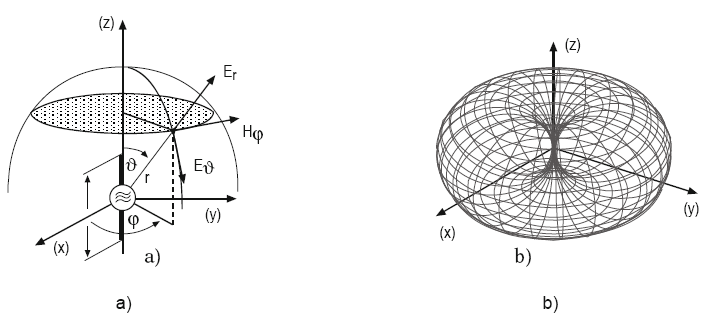
\includegraphics[width=.8\textwidth]{Abbildungen/Kapitel2/Feldverlauf.png}
    \caption[Schematischer Aufbau von Schirmkabinen]{Schematischer Aufbau von Schirmkabinen nach~\cite{EMC-Technik_Stahlblechplatten, EMC-Technik_Sandwichmodul, EM_Schirmung, Design_of_shielded_enclosures}}
    \label{fig:3_Allgemeiner_Aufbau_Schirmkabinen}
\end{figure}

Der Vorteil verschraubter Stahlblechwannen ist offensichtlich die hohe Haltbarkeit der Verschraubung. Allerdings ist die erreichbare Schirmdämpfung sehr sensitiv bezüglich der korrekten Lage der Hochfrequenz"=Dichtungen (HF-Dichtungen) zwischen den Blechplatten. Weiterhin neigen diese Module zum Vibrieren und je nach Größe ist zusätzlich eine Außenkonstruktion für die Selbsttragfähigkeit des Schirmkabine notwendig~\cite{EM_Schirmung}.
\par
\vspace{\linespace}
Ein System aus Verbund- oder Sandwich-Paneelen ist selbsttragend und benötigt aufgrund der überlappenden Profile zwischen den einzelnen Modulen keine HF-Dichtungen. Als Nachteil ist hier vor allem zu nennen, dass die unsachgemäße Verschraubung bei Verwendung selbstschneidender Schrauben zu Lecks führen kann, weil die Anpressung der Profile an die Modulwände stellenweise nicht mehr gegeben ist~\cite{EM_Schirmung}. 
\par
\vspace{\linespace}
Bei vergleichbarer Größe und Ausstattung sind Kabinen aus Sandwich-Modulen im Allgemeinen günstiger als solche aus Stahlblechplatten~\cite{EMC-Technik_Sandwichmodul, EMC-Technik_Stahlblechplatten}. Dies und die Sensitivität der Stahlblechkonstruktion gegenüber der korrekten Lage der HF-Dichtungen waren unter anderem ausschlaggebend für die Wahl der Sandwichbauweise für den Aufbau der Modulwände. Im folgenden \Abschnitt\ref{cha:3_Konzepterstellung} wird auf die Konzeptauswahl näher eingegangen.  %Deshalb und aufgrund der Sensitivität gegenüber der korrekten Lage der HF-Dichtungen soll die Konstruktion im Rahmen dieser Arbeit in Anlehnung an die Sandwich-Modulbauweise erfolgen. 





